% 4

\chapter{Sviluppo}

Quando si vuole sviluppare un’applicazione desktop la prima cosa a cui si pensa è per quale sistema operativo svilupparla, quale linguaggio usare ed opzionalmente a quale base dati si ha bisogno di connettersi.
In questo caso la scelta è caduta su Electron, un framework Open Source sviluppato dal team di GitHub che permette lo sviluppo di app cross platform utilizzando il medesimo approccio di Apache Cordova, ovvero attraverso JavaScript, HTML, e CSS.
Si tratta di un modulo Npm, quindi eredita tutte le API e le funzionalità di Node.js.
\\
Il vero potenziale di Electron è dato dal fatto che si può costruire una desktop app utilizzando qualsiasi libreria scritta in Node.js, rendendolo di fatto uno strumento molto potente anche per interagire con il sistema operativo.
\\
Nello specifico dello sviluppo del sofware, si possono distinguere tre specifiche aree:
\begin{itemize}
	\item Back-End, comprende tutto ciò che riguarda lo sviluppo della logica del software, ovvero cosa fare con i dati, come trattare quelli ricevuti, cosa restituire all'utente.
	\item Front-End, comprende tutto ciò che riguarda l'interfaccia utente, quindi come presentare i dati passati dal Back-End, la grafica, il template, il typewriting, l’accessibilità e l’usabilità.
	\item Packaging dell'App, la creazione del prodotto finale, ovvero il software in versione eseguibile per tutte le tipologie di piattaforme di elaborazione.
\end{itemize}


% 4.1

\section{Sviluppo del Back-End}

Nella struttura di un app basata su Electron, bisogna discutere di due tipi di processo esistenti:
\begin{itemize}
	\item  il processo chiamato \textbf{main} che esegue lo script indicato nel file package.json è il processo principale. Lo script che viene eseguito nel processo principale può visualizzare una \Gls{gui} tramite la creazione di pagine web. Il processo principale crea pagine web mediante la creazione di istanze di BrowserWindow, dove vengono eseguite nel proprio processo di rendering. Quando viene eliminata un'istanza di BrowserWindow, il processo di rendering corrispondente viene anch'esso terminato. Il processo principale quindi, gestisce tutte le pagine web e il corrispondente processo di rendering.
	\item il processo di \textbf{rendering}, invece è il processo che gestisce ogni pagina web, visualizzata tramite Chromium con la sua architettura multi-processo, tale processo è isolato e può occuparsi solo delle pagine web in esecuzione in esso.
	Pertanto nelle pagine web chiamare le API dell'interfaccia grafica nativa non è consentito perché la gestione delle risorse di sistema nelle pagine web è molto pericolosa ed è facile perdere risorse. Se si desidera eseguire operazioni di \Gls{gui} in una pagina web, il processo di rendering della pagina web deve comunicare con il processo principale per richiedere che il processo principale esegua tali operazioni.
\end{itemize}

\begin{figure}[H]
    \centering
    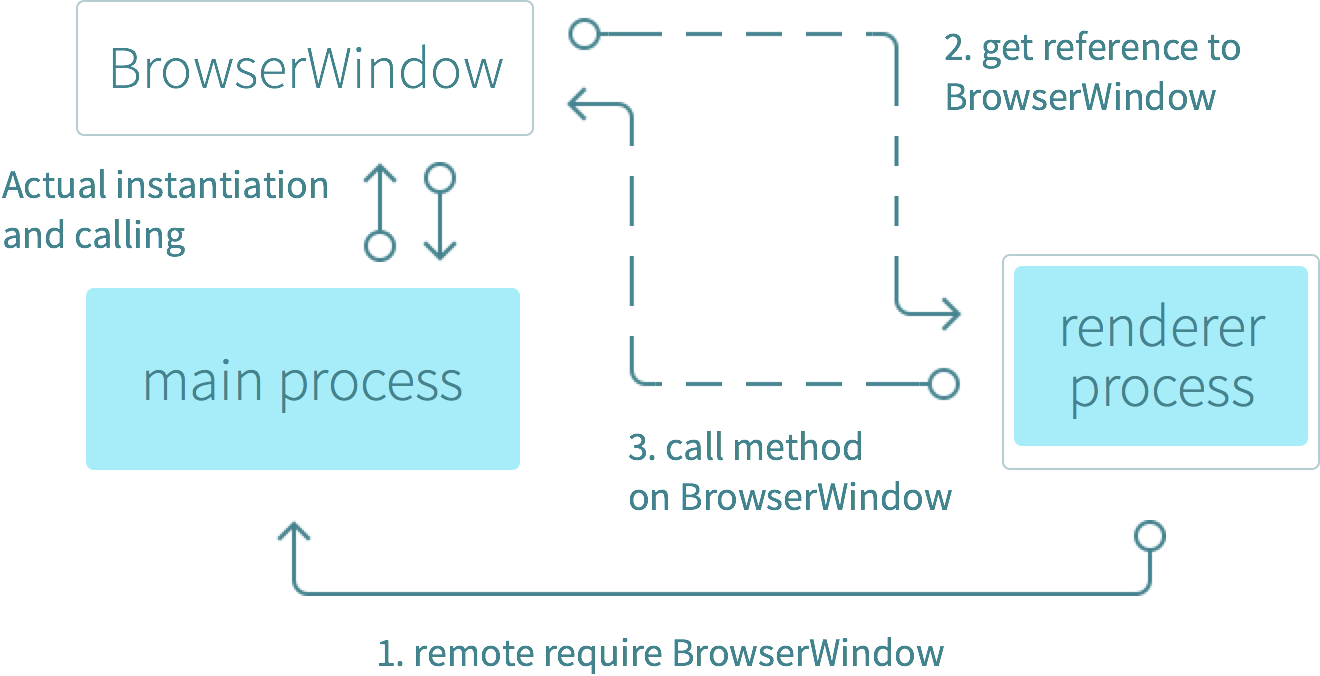
\includegraphics[scale=0.25]{electron-architecture.png}
    \caption{Electron - Architettura di un app}
    \label{fig:ElectronArch}
\end{figure}

% 4.1.1

\subsection{Utilizzo delle API Electron}

Electron offre una serie di API che supportano lo sviluppo di un'applicazione desktop sia nel processo principale che nel processo di rendering. In entrambi i processi, devi accedere alle API di Electron richiedendo il relativo modulo incluso:

\begin{figure}[H]
    \centering
    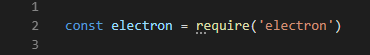
\includegraphics{apiElectron.png}
    \caption{importazione API Electron}
    \label{fig:ApiElectron}
\end{figure}

A tutte le API Electron viene assegnato un tipo di processo. Molti di essi possono essere utilizzati solo dal main, alcuni solo da un processo di rendering, alcuni da entrambi. Ad esempio, una finestra in Electron viene creata utilizzando la classe BrowserWindow, disponibile solo nel processo principale.

\begin{figure}[H]
    \centering
    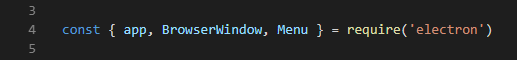
\includegraphics{browserWindow.png}
    \caption{importazione classe BrowserWindow}
    \label{fig:BrowserWindow}
\end{figure}

\begin{figure}[H]
    \centering
    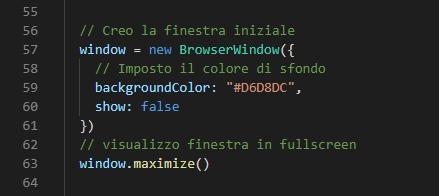
\includegraphics{browserWindow2.png}
    \caption{Creazione BrowserWindow}
    \label{fig:BrowserWindow2}
\end{figure}


% 4.1.2

\subsection {Apertura e salvataggio del progetto}

Durante l'utilizzo del software l'utente deve avere la possibilità attraverso una funzione apposita, di poter salvare un progetto in stato d'opera e/o di leggere un progetto precedentemente salvato.
Per la realizzazione di questa funzionalità, si è scelto di non utilizzare un database ma di un semplice salvataggio dei dati attraverso un file \Gls{json} nel file system della piattaforma di elaborazione in uso.
JSON è un modo per archiviare le informazioni in modo organizzato e di facile accesso per l'utilizzo delle stesse all'interno di una applicazione (web, mobile o di qualsiasi altro tipo).

\begin{figure}[H]
    \centering
    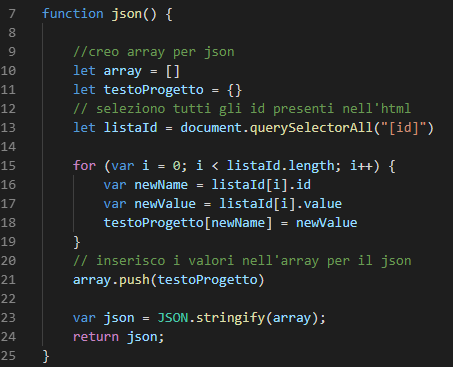
\includegraphics{json.png}
    \caption{Creazione Json}
    \label{fig:json}
\end{figure}

Nella figura ~\ref{fig:json} viene mostrata l'implementazione della funzione "json" per la creazione del file JSON contenente i valori inseriti nel progetto. Inizialmente, utilizzando la funzione querySelectorAll vengono selezionati tutti gli Id contenuti nell'html del main, successivamente, attraverso un ciclo for per l'iterazione degli stessi, vengono inseriti nell'array contenuto nel JSON.

\begin{figure}[H]
    \centering
    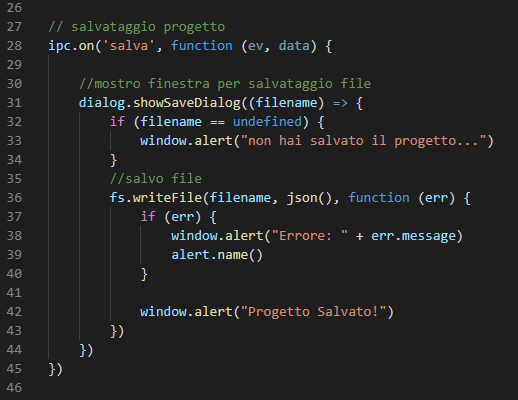
\includegraphics{salvataggio.png}
    \caption{funzione salvataggio}
    \label{fig:salvataggio}
\end{figure}

Electron per comunicare tra processi renderer e main, in entrambe le direzioni, utilizza la comunicazione interprocesso \Gls{ipc}.\\  Come mostrato nella figura ~\ref{fig:salvataggio} la funzione relativa al salvataggio del progetto viene richiamata tramite IPC al messaggio 'salva', e grazie all'utilizzo delle API di Node.js, viene creato all'interno del file system, il file JSON passato dalla funzione "json()" precedentemente illustrata.


% 4.1.3

\newpage

\subsection {Calcolo riclassificazioni e forecast}

Come già visto precedentemente, per l'analisi di bilancio di un'azienda spesso si utilizzano diverse tipologie di riclassificazione, sia per lo stato patrimoniale che per il conto economico. Nel software realizzato si è deciso di mettere a disposizione all'utente, per quanto riguarda lo stato patrimoniale la scelta tra la riclassificazione finanziario, funzionale o entrambe, mentre per il conto economico viene calcolata solo la riclassificazione al valore aggiunto.
Le riclassificazioni calcolate vengono poi usate per calcolare gli indici per il forecast per l'anno di riferimento del progetto.
Per il calcolo delle varie riclassificazioni e forecast sono state realizzate delle specifiche classi Javascript, in cui attraverso l'utilizzo di Jquery per l'acceso al \Gls{dom} e attraverso la funzione importata con la libreria del MaskMoney illustrata precedentemente, vengono applicate tutte le formule del caso.


% 4.1.4

\subsection {Creazione pdf}



% 4.2

\newpage

\section{Sviluppo del Front-End}

Per lo sviluppo di un interfaccia utente efficace si deve tener conto di due aspetti oltre a quello tecnico, che sono:
\begin{itemize}
\item Accessibilità
\item Usabilità
\end{itemize}

L'\textbf{usabilità} è un approccio alla progettazione volto a rendere l'interazione tra il prodotto e l'utente migliore sotto i seguenti aspetti:
\begin{itemize}
    \item Efficacia, cioè permettere agli utenti di raggiungere i loro obiettivi in maniera precisa e completa;
    \item Efficienza, cioè l'ottimizzazione delle risorse impiegate;
    \item Soddisfazione, come libertà dal disagio e attitudine positiva con cui gli utenti raggiungono specifici obiettivi attraverso l’uso del prodotto.
\end{itemize}
Nel web, l'usabilità si pone i seguenti obiettivi:
\begin{itemize}
    \item Presentare l'informazione all'utente in modo chiaro e conciso, evitando termini tecnici o specialistici;
    \item Semplificare la struttura del compito;
    \item Offrire all'utente le scelte corrette, in una maniera che risulti ovvia;
    \item Organizzare ogni pagina in modo che l'utente riconosca la posizione e le azioni da compiere;
    \item Eliminare ogni ambiguità relativa alle conseguenze di un'azione (es. fare clic su cancella/rimuovi/compra);
    \item Mettere la cosa più importante nella posizione giusta della pagina web o dell'applicazione web;
    \item Fare in modo che l'utente abbia un rapido feedback ad ogni azione compiuta, ad esempio la comparsa di un messaggio di successo o errore all'invio di dati con una form;
    \item Rendere la grafica accattivante ed interessante dal punto di vista visivo attraverso l'uso di diagrammi, tabelle, sezioni informative e coordinando bene i colori;
    \item Ridurre gli sforzi cognitivi dell'utente.
\end{itemize}
In generale cercare di rendere il sistema il più semplice possibile da usare, in modo da ridurre al minimo gli sforzi sull'utilizzo del mezzo.

L'\textbf{accessibilità} è un aspetto di fontamentale importanza, specialmente per un gestionale web di una ; il suo scopo è garantire l'accesso alle risorse (prodotti e servizi) da parte di chiunque, siano essi soggetti con disabilità, con scarse competenze informatiche o con dispositivi diversi.
I criteri dell'accessibilità sono quelli delle linee guida del  che attraverso una sua sezione denominata  ha definito i linguaggi e le procedure standard per rendere il Web uno strumento realmente democratico e universale.
Queste direttive sono state percepite in Italia con la Legge "Stanca" (Legge 4/2004) che sancisce obblighi e sanzioni per la  e le aziende appaltate.
In generale i requisiti di accessibilità contenuti nella Legge Stanca e successive modificazioni, contenuti anche in un documento online sul sito del governo , sono i seguenti:
\begin{itemize}
    \item Alternative testuali, obbligatorie per tutte i contenuti non testuali (come immagini, filmati e audio);
    \item Adattabilità, cioè prevedere che i contenuti si adattino a diversi layout in base alla grandezza e al formato dello schermo utente (responsive web design);
    \item Distinguibile, rendere più semplice agli utenti la visione e l'ascolto dei contenuti, separando i contenuti in primo piano dallo sfondo;
    \item Accessibile da tastiera, cioè garantire una buona navigabilità prevedendo un percorso di TAB;
    \item Colori, il contrasto tra le scritte e lo sfondo deve essere chiaro, ma non si devono usare colori discordanti tra loro o lampeggianti che possano causare crisi epilettiche;
    \item Navigabile, fornire una struttura del sito chiara, dove l'utente possa orientarsi e raggiungire qualsiasi sezione attraverso links;
    \item Assistenza per l'inserimento, fornire gli aiuti e le spiegazioni necessarie affinché l'utente sia in grado di compilare correttamente le form del sito;
    \item Compatibilità, il sito deve essere accessibile da tutte le piattaforme e deve utilizzare tecnologie standard.
\end{itemize}

% 4.2.1

\subsection{Tecnologie usate nello sviluppo del front-end}

Mentre per lo sviluppo del back-end abbiamo a disposizione una gran quantità di tecnologie concorrenti per svolgere lo stesso compito, per il front-end le tecnologie di base sono sempre le stesse: \Gls{html}, \Gls{css} e JavaScript.

\textbf{\Gls{html}} è un linguaggio di markup per le pagine web i cui standard sono definiti dal e serve per descrivere il contenuto di una pagina web, sia testuale che multimediale, attraverso dei tag.
Sebbene il linguaggio sia in grado di definire anche regole di formattazione come la centratura del testo o la dimensione dei caratteri, il suo scopo primario è quello di descrivere i contenuti e il loro significato semantico, attraverso l'uso dei tag appropriati (ad esempio \textless p\textgreater  per i paragrafi, \textless h1\textgreater  per un titolo di primo livello, \textless  address\textgreater  per informazioni relative ad un indirizzo, etc.).
Attualmente la versione più recente delle specifiche è chiamata HTML 5 e comporta rispetto alle precedenti versioni l'aggiunta di alcuni tag per gli elementi multimediali, il miglioramento i controlli di input per le form, il controllo della geolocalizzazione e l'intruduzione dello Web Storage come alternativa ai cookies.

\textbf{\Gls{css}}  è il linguaggio usato per definire il layout (impaginazione), la formattazione del testo e l'aspetto grafico in generale; può essere definito sia all'interno della pagina \Gls{html} che all'esterno come file a sé stante, che è generalamente la scelta migliore.
Nel nostro caso sono state usate alcune delle proprietà più recenti del linguaggio come la box-shadow o la border-radius appartenenti alle specifiche CSS 3.
Per mantenere la compatibilità tra i differenti browser (e nei limiti del possibile anche con le versioni più vecchie degli stessi) sono state applicate ad ogni proprietà CSS 3 delle tecniche di cross-browsing, cioè la riscrittura della stessa proprietà in modi differenti, vedi figure ~\ref{fig:Css3Shadow} e ~\ref{fig:Css3Radius}.

\begin{figure}[H]
    \centering
    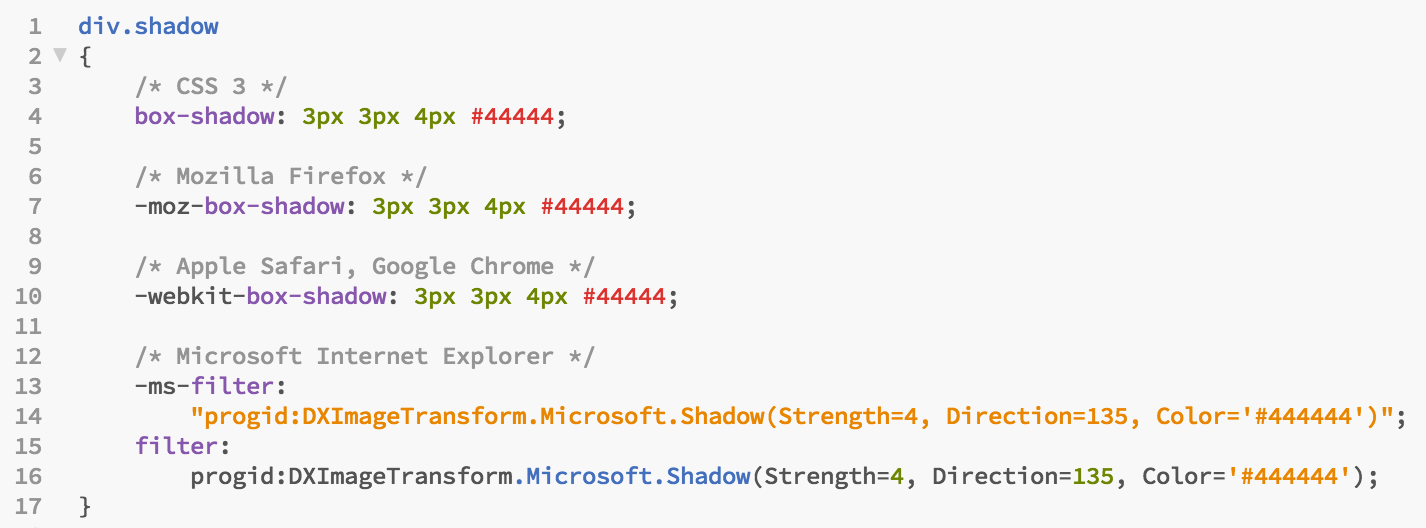
\includegraphics[scale=0.5]{css3-1.png}
    \caption{CSS 3 text-shadow cross-browser}
    \label{fig:Css3Shadow}
\end{figure}

\begin{figure}[H]
    \centering
    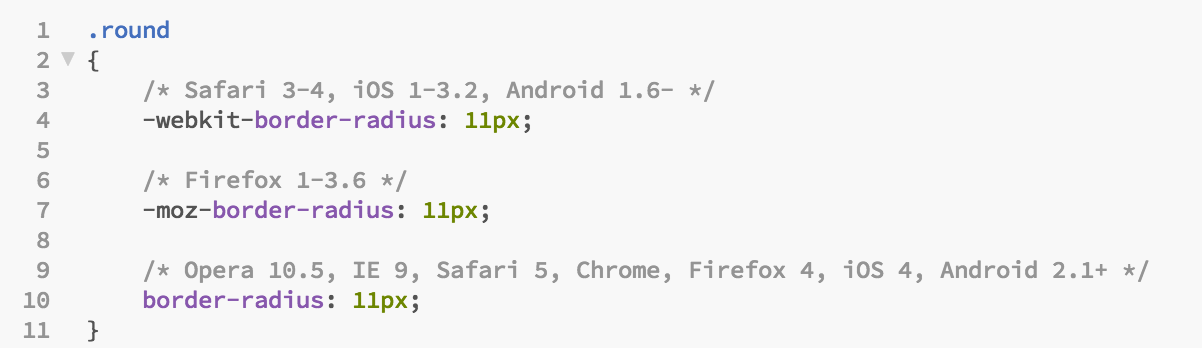
\includegraphics[scale=0.5]{css3-2.png}
    \caption{CSS 3 border-radius cross-browser}
    \label{fig:Css3Radius}
\end{figure}

\textbf{JavaScript} è un linguaggio di scripting adatto per creare effetti dinamici interattivi basati su eventi, come il click di un bottone, la selezione di una voce da una tendina, la pressione di un tasto o il caricamento di una pagina.
Anche se con il javascript è possibile creare applicazioni vere e proprie si deve sempre tener conto che è un linguaggio accessorio, ovvero c'è la possibilità per l'utente di disabilitarlo, specialmente nel caso si abbia delle disabilità o dei problemi di visualizzazione.
Pertanto nessuna funzionalità deve contare unicamente su javascript per funzionare, ma il suo uso è comunque consigliato per aumentare l'esperienza utente (quegli obiettivi dell'usabilità esposti sopra) ad esempio prevedendo dei messaggi di errore nel caso si inseriscano dei valori errati nei campi, o un calendario all'immissione di un campo data, o anche per sostituire delle proprietà del CSS 3 nel caso il browser dell'utente non la supporti (i cosiddetti polyfill).

\textbf{jQuery}  è una libreria Javascript molto diffusa il cui scopo è semplificare la selezione, la gestione e la manipolazione degli eventi, mantenendo però anche la possibilità di utilizzare il linguaggio nella vecchia maniera.
L'uso di jQuery non aggiunge quindi nessuna funzionalità, rende solamente più semplice l'utilizzo del linguaggio e quindi più elevata la produttività del programmatore, non a caso il suo motto è "Write less, do more", anch'essa è stata inclusa nella nostra applicazione web e gli script personalizzati fanno tutti riferimento alla sua sintassi.

 è un'altra tecnologia molto importante per migliorare l'esperienza utente, perché permette di aggiornare il contenuto di una pagina dinamicamente senza effettuare il "refresh" e quindi caricando solo le informazioni necessarie, anziché tutta la pagina.
Si tratta, più che di un nuovo linguaggio, di un insieme di tecniche che fanno uso delle tecnologie sopra descritte, quindi JavaScript per inviare le richieste asincrone e XML o JSON per ricevere le risposte dal server sottoforma di oggetti.
Questa tecnica è stata utilizzata nella nostra applicazione web nella fase di autenticazione post-Cohesion, dove viene richiesto all'utente di scegliere un ruolo da una tendina e automaticamente sulla base di questa scelta viene popolata la tendina delle riferite a quel ruolo.
Un altro utilizzo è nella pagina di inserimento di un nuovo utente, dove a seguito della digitazione di almeno 3 caratteri in una casella di testo, compare un menù di autocomplete che suggerisce i possibili nomi degli utenti cercati.

\textbf{Razor}  infine, è un linguaggio di programmazione lato server, specifico del framework ASP.NET MVC, ma è stato incluso in questa sezione perché serve a descrivere, insieme all'HTML, il contenuto di una View.
Una View che contiene codice Razor sarà un file di tipo .cshtml (nel caso il linguaggio lato server utilizzato sia il C).
Questo linguaggio può utilizzare molte delle classi del framework, semplicemente includendo il namespace nella pagina, ma il suo scopo principale è quello di posizionare gli elementi del Model nella View, passati dal Controller, eventualmente anche iterando una Collection affinché venga stampata a schermo una serie di elementi per ogni elemento della Collection, come in Figura ~\ref{fig:Razor}.

\begin{figure}[H]
    \centering
    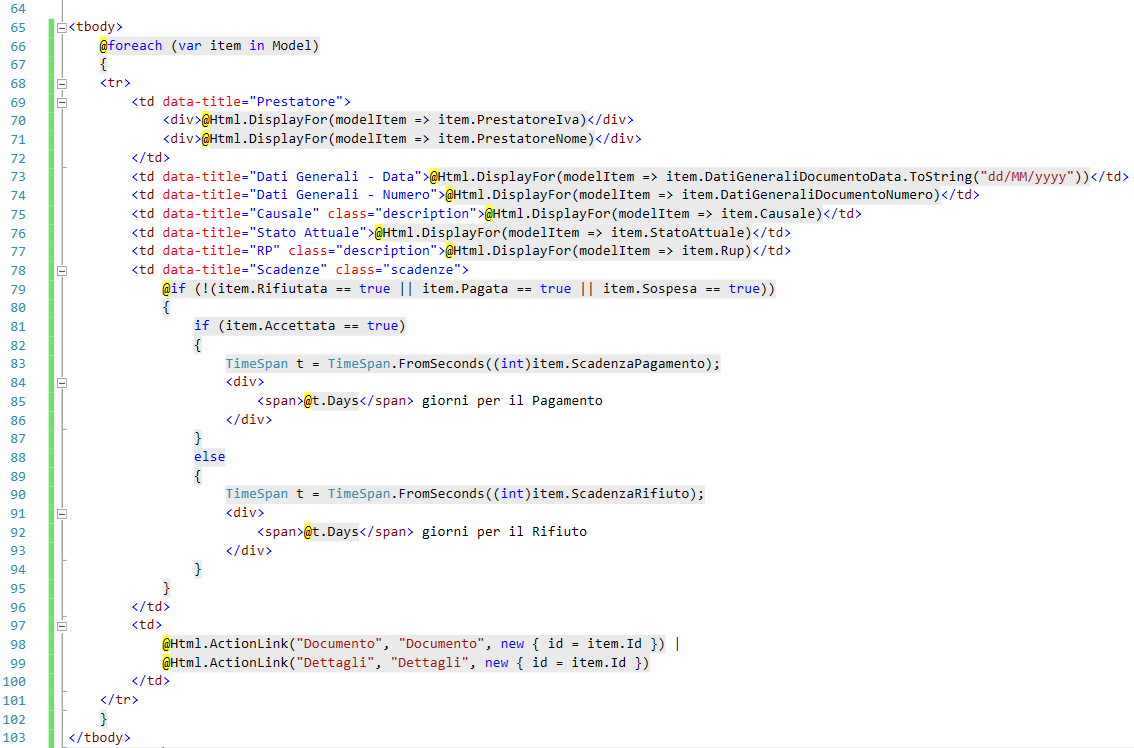
\includegraphics[scale=0.5]{razor-1.png}
    \caption{Esempio di codice Razor per la stampa degli elementi di una collection come righe di una tabella HTML}
    \label{fig:Razor}
\end{figure}


% 4.3

\newpage

\section{Packaging dell'applicazione}

Per lo sviluppo di un interfaccia utente efficace si deve tener conto di due aspetti oltre a quello tecnico, che sono:
\begin{itemize}
\item Accessibilità
\item Usabilità
\end{itemize}

L'\textbf{usabilità} è un approccio alla progettazione volto a rendere l'interazione tra il prodotto e l'utente migliore sotto i seguenti aspetti:
\begin{itemize}
    \item Efficacia, cioè permettere agli utenti di raggiungere i loro obiettivi in maniera precisa e completa;
    \item Efficienza, cioè l'ottimizzazione delle risorse impiegate;
    \item Soddisfazione, come libertà dal disagio e attitudine positiva con cui gli utenti raggiungono specifici obiettivi attraverso l’uso del prodotto.
\end{itemize}
Nel web, l'usabilità si pone i seguenti obiettivi:
\begin{itemize}
    \item Presentare l'informazione all'utente in modo chiaro e conciso, evitando termini tecnici o specialistici;
    \item Semplificare la struttura del compito;
    \item Offrire all'utente le scelte corrette, in una maniera che risulti ovvia;
    \item Organizzare ogni pagina in modo che l'utente riconosca la posizione e le azioni da compiere;
    \item Eliminare ogni ambiguità relativa alle conseguenze di un'azione (es. fare clic su cancella/rimuovi/compra);
    \item Mettere la cosa più importante nella posizione giusta della pagina web o dell'applicazione web;
    \item Fare in modo che l'utente abbia un rapido feedback ad ogni azione compiuta, ad esempio la comparsa di un messaggio di successo o errore all'invio di dati con una form;
    \item Rendere la grafica accattivante ed interessante dal punto di vista visivo attraverso l'uso di diagrammi, tabelle, sezioni informative e coordinando bene i colori;
    \item Ridurre gli sforzi cognitivi dell'utente.
\end{itemize}
In generale cercare di rendere il sistema il più semplice possibile da usare, in modo da ridurre al minimo gli sforzi sull'utilizzo del mezzo.

L'\textbf{accessibilità} è un aspetto di fontamentale importanza, specialmente per un gestionale web di una ; il suo scopo è garantire l'accesso alle risorse (prodotti e servizi) da parte di chiunque, siano essi soggetti con disabilità, con scarse competenze informatiche o con dispositivi diversi.
I criteri dell'accessibilità sono quelli delle linee guida dche attraverso una sua sezione denominata ha definito i linguaggi e le procedure standard per rendere il Web uno strumento realmente democratico e universale.
Queste direttive sono state percepite in Italia con la Legge "Stanca" (Legge 4/2004) che sancisce obblighi e sanzioni per e le aziende appaltate.
In generale i requisiti di accessibilità contenuti nella Legge Stanca e successive modificazioni, contenuti anche in un documento online sul sito del governsono i seguenti:
\begin{itemize}
    \item Alternative testuali, obbligatorie per tutte i contenuti non testuali (come immagini, filmati e audio);
    \item Adattabilità, cioè prevedere che i contenuti si adattino a diversi layout in base alla grandezza e al formato dello schermo utente (responsive web design);
    \item Distinguibile, rendere più semplice agli utenti la visione e l'ascolto dei contenuti, separando i contenuti in primo piano dallo sfondo;
    \item Accessibile da tastiera, cioè garantire una buona navigabilità prevedendo un percorso di TAB;
    \item Colori, il contrasto tra le scritte e lo sfondo deve essere chiaro, ma non si devono usare colori discordanti tra loro o lampeggianti che possano causare crisi epilettiche;
    \item Navigabile, fornire una struttura del sito chiara, dove l'utente possa orientarsi e raggiungire qualsiasi sezione attraverso links;
    \item Assistenza per l'inserimento, fornire gli aiuti e le spiegazioni necessarie affinché l'utente sia in grado di compilare correttamente le form del sito;
    \item Compatibilità, il sito deve essere accessibile da tutte le piattaforme e deve utilizzare tecnologie standard.
\end{itemize}
